%----------------------------------------------------------------------------------------
%	PACKAGES AND OTHER DOCUMENT CONFIGURATIONS
%----------------------------------------------------------------------------------------

\documentclass[fleqn,10pt]{SelfArx} % Document font size and equations flushed left
%\usepackage{lipsum} % Required to insert dummy text. To be removed otherwise
\usepackage{mathrsfs} % para formato de letra
\usepackage[spanish,es-tabla]{babel}
%\usepackage[utf8]{inputenc}

%----------------------------------------------------------------------------------------
%	COLUMNS
%----------------------------------------------------------------------------------------
\setlength{\columnsep}{0.55cm} % Distance between the two columns of text
\setlength{\fboxrule}{0.75pt} % Width of the border around the abstract

%----------------------------------------------------------------------------------------
%	COLORS
%----------------------------------------------------------------------------------------
\definecolor{color1}{RGB}{0,0,90} % Color of the article title and sections
\definecolor{color2}{RGB}{0,20,20} % Color of the boxes behind the abstract and headings

%----------------------------------------------------------------------------------------
%	HYPERLINKS
%----------------------------------------------------------------------------------------
\usepackage{hyperref} % Required for hyperlinks
\hypersetup{hidelinks,colorlinks,breaklinks=true,urlcolor=color2,citecolor=color1,linkcolor=color1,bookmarksopen=false,pdftitle={Title},pdfauthor={Author}}

%----------------------------------------------------------------------------------------
%	ARTICLE INFORMATION
%----------------------------------------------------------------------------------------
\JournalInfo{Tarea, 1, 2020} % Journal information
\Archive{Ezequiel Remus} % Additional notes (e.g. copyright, DOI, review/research article)
\PaperTitle{Tarea 1} % Article title

\Authors{Ezequiel Remus\textsuperscript{1}*} % Authors
%\affiliation{\textsuperscript{1}\textit{Department of Biology, University of Examples, London, United Kingdom}} % Author affiliation
%\affiliation{\textsuperscript{2}\textit{Department of Chemistry, University of Examples, London, United Kingdom}} % Author affiliation
\affiliation{*\textbf{Mail}: ezequielremus@gmail.com} % Corresponding author

\Keywords{} % Keywords - if you don't want any simply remove all the text between the curly brackets
\newcommand{\keywordname}{Keywords} % Defines the keywords heading name

%----------------------------------------------------------------------------------------
%	ABSTRACT
%----------------------------------------------------------------------------------------

\Abstract{
	Durante el asedio a una fortaleza tenemos una catapulta a una distancia horizontal $D$ de
la torre más alta del castillo, de altura $H$. La catapulta se utiliza para lanzar proyectiles y se
puede modelar como un dispositivo mediante el cual cada proyectil parte desde la posición \textbf{(1)} con
velocidad nula, luego se mueve sobre la trayectoria circular de radio R con una aceleración angular
$\ddot{\varphi} = -K {\varphi}^2$
(donde $K > 0$ es un valor que puede controlar el soldado que opera la catapulta1
) y
finalmente se puede liberar ya sea en la posición \textbf{(2)} (${\varphi} = \frac{\pi}{3})$ o en la posición \textbf{(3)}.
\begin{itemize}
\item[a) ] Expresá la velocidad tangencial v del proyectil cuando está en la catapulta en función de
$K$, $R$ y $\varphi$.
\item[b) ] La catapulta se libera en la posición $(2)$. Calculár en función de $R$, $g$, $D$ y $H$ el valor que
debe darle a $K$ el operador de la catapulta para que el proyectil impacte justo en el punto
$P$ en la torre. ¿Existe siempre un $K$ para cualquier valor de los otros parámetros que haga
que el proyectil impacte en $P$? Si no es así, discutí el (los) caso(s) límite(s) y su significado
físico.
\item[c) ]  Si quieren que el proyectil impacte en $P$, ¿Por qué no eligen liberarlo en el punto (3)? ¿Qué
problema fundamental se presenta? Justificá sin hacer cuentas
\end{itemize}

}
%----------------------------------------------------------------------------------------

%%%%%%%%%%%%%%%%%%%%%%%%%%%%%%%%%%%%%%%%%%%%%%%%%%%%%%%%%%%%
%			 	  Definciciones de Variables               %
%%%%%%%%%%%%%%%%%%%%%%%%%%%%%%%%%%%%%%%%%%%%%%%%%%%%%%%%%%%%
%%%%%%%%%%%%%%%%%%%%%
%     COLORES       %
%%%%%%%%%%%%%%%%%%%%%
\definecolor{R}{RGB}{176, 11, 11}
\definecolor{B}{RGB}{52, 75, 201}
\definecolor{G}{RGB}{20, 176, 18}
\definecolor{M}{RGB}{133, 71, 33}

%%%%%%%%%%%
%  TEXTO  %
%%%%%%%%%%%
\newtheorem{teo}{Teorema}[subsection]
\newtheorem{cor}{Corolario}[subsection]
\newtheorem{defi}{Definición}[subsection]
\newtheorem{obs}{Observación}[subsection]
\newtheorem{propo}{Proposición}[subsection]
\newtheorem{prop}{Propiedad}[subsection]
\newtheorem{ej}{Ejercicio}[subsection]

%%%%%%%%%%%%%%%%%%
%  MATEMATICAS   %
%%%%%%%%%%%%%%%%%%
% Este comando es para conjuntos numericos. Ej: \conj{R}
\newcommand{\conj}[1]{$\mathbb{#1}$ }
% Vectores
\newcommand{\vecAn}[1]{{$(a_1,a_2,\cdots,a_n )$ #1}}
\newcommand{\vecBn}[1]{{$(b_1,b_2,\cdots,b_n )$ #1}}
\newcommand{\vecdos}[2]{{(#1,#2)}}
\newcommand{\vectres}[3]{{(#1,#2,#3)}}
\newcommand{\dom}[1]{{\mathcal{D}}}
\newcommand{\origen}[1]{{$\mathcal{O}$}}
\newcommand{\modulo}[1]{{\vert{#1}\vert}}
\newcommand{\norma}[1]{{\Vert{#1}\Vert}}
\newcommand{\prodesc}[2]{{\langle #1,#2 \rangle}}
\newcommand{\cuerpo}[1]{\textbf{#1}}

\newcommand{\titulo}[1]{\subsection{\underline{\textbf{\color{B}{#1}}}}}
\newcommand{\ejercicio}[1]{\subsection{\textbf{\color{R}{#1}}}}
\newcommand{\solucion}[1]{\fbox{\textbf{Solución}}#1}
\newcommand{\resultado}[1]{\color{G}{#1}}
\newcommand{\sii}{\Longleftrightarrow}
\newcommand{\azul}[1]{\color{blue}{#1}}
\newcommand{\rojo}[1]{\color{red}{#1}}
\begin{document}

\flushbottom % Makes all text pages the same height
\maketitle % Print the title and abstract box
\tableofcontents % Print the contents section
\thispagestyle{empty} % Removes page numbering from the first page

%----------------------------------------------------------------------------------------
%	ARTICLE CONTENTS
%----------------------------------------------------------------------------------------

\section*{Introduction y Obvservaciones Iniciales} % The \section*{} command stops section numbering

\addcontentsline{toc}{section}{Introduction y Obvservaciones Iniciales} % Adds this section to the table of contents

%------------------------------------------------
Es necesario hacer un par de anotaciones iniciales: 
\begin{figure}[h] % Using \begin{figure*} makes the figure take up the entire width of the page
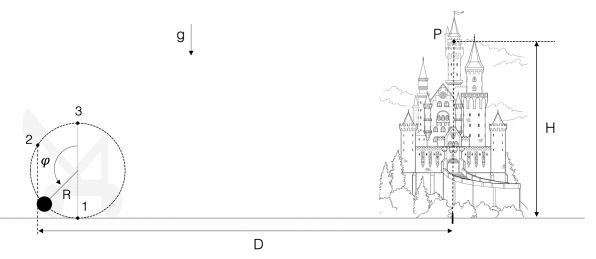
\includegraphics[scale=0.5]{figuras/fig1.jpg}
\caption{Esquema Del problema}
\label{fig:1}
\end{figure}

\begin{enumerate}
\item Como el proyectil al moverse sobre la catapulta lo hace sobre una trayectoria circular de radio constante $R$, 
entonces sobre la catapulta solo tendremos presente un movimiento circular con coordenadas puramente tangenciales, lo cual se debe a que 
$\dot{r} = \frac{d}{dt}(R) = 0$
\item Al ver la particularidad anterior y como nos dan una aceleracion angular, lo mas probable que sea conveniente describir el movimiento en coordenadas polares.
\item Como me dice que la velocidad en el punto \textbf{(1)} es nula (y estamos parados en un movimiento puramente circular en esta instancia), vale aclarar que como $\overline{v} = \dot{R} \hat{r} + R \dot{{\varphi}} \hat{{\varphi}}$, para que esta velocidad en el incicio sea nula, debe pasar que: \[\overline{v} = 0 = \dot{R} \hat{r} + R \dot{{\varphi}} \hat{{\varphi}} \]
Luego, por lo dicho en la primer observacion, la componente radial de la ecuación es cero. Entonces, debe pasar que:
\[0 = R \dot{{\varphi}} \hat{{\varphi}} \sii 0 = \dot{{\varphi}}\]
Pues, $R$ es un valor real.
\item Uno de los puntos importantes en este ejercicio es el punto \textbf{(2)}. Este punto se encuentra a una altura respecto al piso. 

Como ya sabemos, el radio es constante, por lo que el diametro de la catapunta es $2R$. Sabemos del enunciado que esl punto \textbf{(2)} se ubica en el ángulo ${\varphi}_2 = \frac{\pi}{3}$ segun el siguiente sistema de coordenadas
\begin{figure}[h] 
\centering
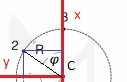
\includegraphics[scale=0.8]{figuras/fig3.jpg}
\caption{Coordenadas Cartesianeas para la Catapulta}
\label{fig:3}
\end{figure}
Nuestro objetivo es calcular el lado $C$ el cual se corresponde con el cateto adyacente del triangulo rectangulo formado por $R$ (la hipotenusa), $C$(cateto adyacente) y su otro cateto. Pero esto es facil de hacer, porque de pitagoras sabemos que el cateto adyacente lo podemos calcular como:
\[\sin{\varphi} = \frac{C}{R} \overbrace{\Longrightarrow}^{\varphi = \pi/3} \frac{\sqrt{3}}{2} = \frac{C}{R} \sii C = \frac{\sqrt{3}}{2} R\] 
Luego, la altura del punto \textbf{(2)} respecto del piso es:
\[h_0 = R + C = R + \frac{\sqrt{3}}{2} R = \frac{2}{2} R + \frac{\sqrt{3}}{2} R = \azul{\sqrt{3} R}\] 

\end{enumerate}


\section{Solucion al Inciso (a)}
Tomemos el siguiente sistema de referencia para estudiar el movimiento de el proyectil sobre la catapulta:


\begin{figure}[h] % Using \begin{figure*} makes the figure take up the entire width of the page
\centering
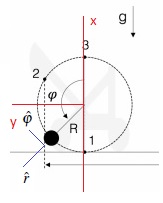
\includegraphics[scale=0.8]{figuras/fig2.jpg}
\caption{Coordenadas Cartesianeas y Polares definidas}
\label{fig:2}
\end{figure}

Como se ve en la figura, tomamos que el movimiento de la catapulta tiene en cuenta que, para $t=t_0=0$, ${\varphi}(t_0) = \pi$ y que ${\varphi}(t_f) =0$ (Por como tomamos las coordenadas)

Además debemos recordar que $v(t_0)=0$ definido asi en el problema. 

Por otro lado, recordando la definicion de velocidad en polares, la velocidad tangencial, la cual es la que nos piden, esta definida como:
\begin{equation}
v_t = r \dot{\varphi} \hat{\varphi}
\end{equation}
 Entonces, lo único que necesitamos calrular, para conocer la velocidad tangencial, sera  $\dot{\varphi}$. Esto lo hacemos integrando la aceleración angular dada al inicio la cual tiene equación $\ddot{\varphi} = - K {\varphi}^2$

\[\ddot{\varphi} = \frac{d \dot{\varphi}}{dt} = \frac{d \dot{\varphi}}{d{\varphi}} \frac{d{\varphi}}{dt}= \dot{\varphi} \frac{d \dot{\varphi}}{d{\varphi}}\]

Luego, teniendo en cuenta este resultado vemos que:
\[\ddot{\varphi} = - K {\varphi}^2 = \dot{\varphi} \frac{d{\dot{\varphi}}}{d{\varphi}}\]
\[\Rightarrow \int_{\pi}^{{\varphi}_f} - K {\varphi}^2 d{\varphi} = \int_{0}^{\dot{\varphi}_f} \dot{\varphi} d \dot{\varphi} \sii \]
\[\left[ -K \frac{{\varphi}^3}{3}\right]_{\pi}^{{\varphi}_f} = \frac{{\dot{\varphi}_f}^2}{2} \sii  \frac{-K}{3} \left[{\pi}^3-{{\varphi}_f}^3\right] = \frac{{\dot{\varphi}_f}^2 - {\dot{\varphi}_0}^2}{2}\]

Por lo que la ecuación para ${\dot{\varphi}}$ se despeja de el resultado anterior, quedando:
\begin{equation}
\azul{\dot{\varphi}_f = \sqrt{{\dot{\varphi}_0}^2 - \frac{2}{3} K \left[{{\varphi}_f}^3 - {\pi}^3\right]}}
\end{equation}

Como parte desde el punto \textbf{(1)} con velocidad nula, tenemos que $\dot{\varphi}_0=0$ (Como se noto en la sección anterior)
Por lo tanto, usando la ecuación \textbf{2} en la ecuacion para la ecuación de la velocidad tangencial, se tiene que:
\begin{equation}
\rojo{v_t = R \sqrt{ - \frac{2}{3} K \left[ {{\varphi}_f}^3 - {\pi}^3 \right]}}
\end{equation}

Veamos si este resultado tiene sentido, ya que a simple vista tenemos algo negativo dentro de la raiz, fijemonos cuando el termino que esta dentro de la raiz es positivo.
\[- \frac{2}{3} K \left[{{\varphi}_f}^3 - {\pi}^3\right] > 0 \sii - \frac{2}{3} K {{\varphi}_f}^3 + \frac{2}{3} K {{\pi}_f}^3 > 0\]
\[ \frac{2}{3} K {{\pi}_f}^3 > \frac{2}{3} K {{\varphi}_f}^3 \sii \azul{{\pi}_f > {\varphi}_f}\]
Lo cual tiene sentido para como planteamos las coordenadas en el dibujo.

\section{Solucion al Inciso (b)}
En esta parte del ejercicio, nos piden que valores de $K$ existen para que al salir de la posición \textbf{(2)} el proyectil caiga justo en el punto $P$ indicado en la \textit{figura}(\ref{fig:1}) el cual se encuentra a una altura $H$ respecto del piso y a una distancia $D$ respecto de la catapulta, o sea $P(x,y) = (D, H)$. 

Es necesario conocer de que altura sale el proyectil, ya que este sera nuestro valor de altura inicial de salida, esto es por como tomaremos las coordenadas para la solución de este inciso. Esta altura la calculamos en la seccion de observaciones en la cual obtuvimos que $h_0 = \sqrt{3} R$. 

Acorde a como tomamos el sistema de referencia, el punto de partida sera $(x_0,y_0) = (0, \sqrt{3} R)$. 

\begin{figure}[h] % Using \begin{figure*} makes the figure take up the entire width of the page
\centering
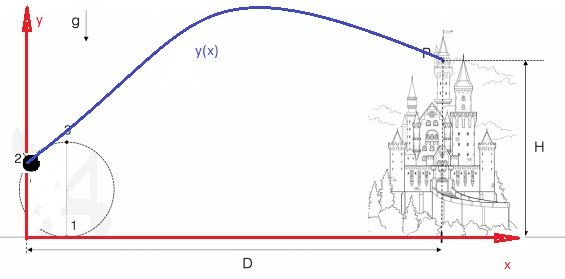
\includegraphics[scale=0.5]{figuras/fig5.jpg}
\caption{Sistema de Referencia tomado para describir $y(x)$ (la trayectoria dibujada es solo ilustrativa, no la real)}
%\label{fig:2}
\end{figure}

A partir de este punto, el proyectil se deja en viaje libremente con un vector velocidad inicial (cuyo valor lo calcularemos a partir de la ecuacion (3) obtenida anteriormente) que debe descomponerse en sus coordenadas $(x,y)$, ya que como savemos, el vector velocidad en su posicion inicial tiene una dirección orientada a $\frac{\pi}{3}$ respecto de la horizontal.
Luego, a partir de esta aclaración, debemos descomponer el movimiento del proyectil a partir de dos movimientos, uno rectilineo uniforme respecto de la horizontal y otro de caida libre respecto de el eje vertical debido a la presencia de la gravedad ($g$). 

Calculemos primero con que velocidad sale disparado el proyectil. Sabemos que ${\varphi}_2 = \frac{\pi}{3}$ (ángulo dado en el problema). Reemplazando esto en la ecuación obtenida para la velocidad, tenemos que:

\[v_0 = R \sqrt{ - \frac{2}{3} K \left[ \left(\frac{\pi}{3}\right)^3 - {\pi}^3  \right]} = R \sqrt{ \frac{4}{9} {\pi}^3} K 	= \azul{\frac{2}{3} R  \sqrt{ {\pi}^3} K}\] 

Luego, esta velocidad sera el modulo de la velocidad inicial.

Como sabemos, en el punto \textbf{(2)}, el valor de ${\varphi}_2 = \frac{\pi}{3}$ que, trasponiendo esta horientacion con la horizontal en el sentido del movimiento, nos da que la horientación de la velocidad inicial tendra el mismo angulo de salida. Por lo que:
\[\textbf{v} = (|\textbf{v}| \cos{\theta}, |\textbf{v}| \sin{\theta})\]
Como queremos la velocidad inicial:  
\[ v_{0} = (v_{0x}, v_{0y} ) = (|v_0| \cos{\frac{\pi}{3}}, |v_0| \sin{\frac{\pi}{3}})\]
Como dijimos antes, el movimiento debe descomponerse en las siguientes componentes:
\[\left[ \begin{array}{lll}
 x(t) = x_0 + v_{0x} t & \Rightarrow & x(t) = |v_0| \cos{\frac{\pi}{3}} t\\
 y(t) = y_0 + v_{0y} t - \frac{1}{2} g t^2  & \Rightarrow & y(t) = \sqrt{3}R + |v_0| \sin{\frac{\pi}{3}} t - \frac{1}{2} g t^2
\end{array}\right. \]
Notar, que nos referimos a $|v_0|$ como el resultado obtenido anteriormente, es decir: $|v_0| = \frac{2}{3} R  \sqrt{ {\pi}^3} K$

A partir de estos resultados podemos obtener la ecuación de la trayectoria, es decir la composición $y(x)$. Veamos esto:

\[x(t) = |v_0| \cos{\frac{\pi}{3}} t \overbrace{\sii}^{x(t)=D} t = \frac{D}{|v_0| \cos{\frac{\pi}{3}}}\]

Luego, usamos este resultado para componer $y(x(t))$:
\[y(x(t)) = \sqrt{3}R + |v_0| \sin{( \frac{\pi}{3} )} \frac{x(t)}{|v_0| \cos{( \frac{\pi}{3}} ) } - \frac{1}{2} g \left( \frac{x(t)}{|v_0| \cos{( \frac{\pi}{3} )}}\right)^2\]

Usando propiedades trigonometricas y que $x(t_e)=D$ ($t_e = $ \textit{tiempo de encuentro con P}):

\[H = y(D) = \sqrt{3}R + \tan{( \frac{\pi}{3} )} D - \frac{g D^2}{2 |v_0|^2}  \left(1 + \tan^2{( \frac{\pi}{3} )}  \right)\]

Remplazando el valor de $|v_0|$:

\[H  = \sqrt{3}R + \tan{( \frac{\pi}{3} )} D - \frac{g D^2}{2 \left(\frac{2}{3} R  \sqrt{ {\pi}^3} K \right)^2}  \left(1 + \tan^2{( \frac{\pi}{3} )}  \right)\]

Ahora, tratemos de despejar el valor de $K$ y ver si podemos sacar alguna conclusión. Teniendo en cuenta que $\tan{( \frac{\pi}{3} )} =  \sqrt{3}$ y que $\tan^2{( \frac{\pi}{3} )} = (\tan{(( \frac{\pi}{3} )})^2 = (\sqrt{3})^2 = 3$, tenemos que:

\[H  = \sqrt{3}R + \sqrt{3} D - \frac{g D^2}{\frac{8}{9} R^2 {\pi}^3 K^2 }  4 =  \sqrt{3}(R +  D) - \frac{9}{2} \frac{g D^2}{ R^2 {\pi}^3 K^2 }  \sii \]
\[ \sii \frac{9}{2} \frac{g D^2}{ R^2 {\pi}^3 K^2 } = \sqrt{3}(R +  D) - H \sii\]
 \[ \sii \frac{9}{2} \frac{g D^2}{ R^2 {\pi}^3 } =K^2 \left( \sqrt{3}(R +  D) - H \right) \sii\]
\[\sii \frac{9}{2} \frac{g D^2}{ R^2 {\pi}^3 } \frac{1}{\left( \sqrt{3}(R +  D) - H \right)} =K^2  \sii \]
\[\sii \sqrt{\frac{9}{2} \frac{g D^2}{ R^2 {\pi}^3 } \frac{1}{\left( \sqrt{3}(R +  D) - H \right)}} =K \sii\]
\begin{equation}
\rojo{ K = \frac{3 \sqrt{2} D}{2 R} \sqrt{\frac{g}{\sqrt{3}{\pi}^3(R+D)} - \frac{g}{H}}}
\end{equation}
Como vemos en la ecuación \textbf{(4)}, necesitamos que:
\[\frac{g}{\sqrt{3}{\pi}^3(R+D)} - \frac{g}{H} > 0\]
Pues, sino, esto no tendria sentido. Veamos en que condiciones pasa esto:
\[\frac{g}{\sqrt{3}{\pi}^3(R+D)}  >  \frac{g}{H} \sii \frac{1}{\sqrt{3}{\pi}^3(R+D)}  >  \frac{1}{H} \sii \]
\begin{equation}
 \sii \azul{\sqrt{3}{\pi}^3(R+D)  <  H}  
\end{equation}

\paragraph{¿Que nos dice la expreción \textbf{(5)}?}{

Bueno, basicamente lo que nos dice es que debe cumplirse dicha relación para que exista un $K$ talque el proyectil de en el blanco deseado el cual es el punto $P(x,y)=(D,H)$ partiendo de la altura correspondiente y saliendo disparado en el ángulo indicado por el punto \textbf{(2)}. Notemos que depende el radio de la catapulta $R$, de la distancia a la cual esta situada la catapulta respecto del castillo y de una constante. 

Pensemos, lo que nos dice es que, si la altura del punto $P$ fuese menor a $\sqrt{3}{\pi}^3(R+D)$ no existe un valor de $K$ positivo disparado en tales condiciones que pueda dar con $P$, y lo que pasaria es que el ``proyectil seguiria de largo o pegaria en una altura mayor siempre que a la que estaria situado $P$". Es decir, \textit{el proyectil pasaria siempre por encima del punto}.
}

Luego, la expreción \textbf{(4)} nos da los valores de $K$ posibles, siendo estos unicós para cada valores dependiendo de los valores de $R$, $D$ y $H$ y teniendo en cuenta que esta ecuación tiene sentido si se cumple la relacion \textbf{(5)}

\begin{figure*}[ht] % Using \begin{figure*} makes the figure take up the entire width of the page
\centering
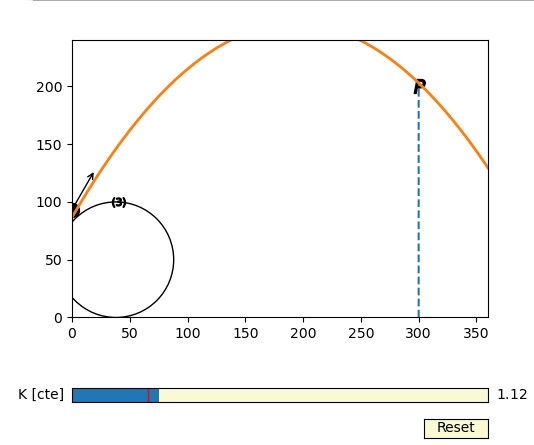
\includegraphics[scale=0.5]{figuras/fig4.jpg}
\caption{Trayectoria del Proyectil}
%\label{fig:2}
\end{figure*}

\section{Solucion al Inciso (c)}
Nos preguntan porque no lo disparan del punto \textbf{(3)} en vez de en el punto \textbf{(2)}.

Se puede notar que al dispararlo del punto \textbf{(3)}, el vector velocidad queda en dirección Horizontal, es decir, \textit{paralelo al piso}. Luego, como el movimiento del proyectil a partir de este punto, como dijimos anteriormente, se descompone en las coordenadas horizontal y vertical. 

Luego, no existe ningun valor de $K$ que haga que el proyectil de en el blanco deseado(osea en el punto $P$). Esto se debe a que el proyectil saldra disparado de una altura $2R$ desde la catapulta y solo podra alcanzar dicha altura ($2R$), si y solo si no existiese gravedad o la velocidad horizontal dada sea tal que el efecto de la gravedad sea despreciable respecto a la velocidad dada en la componente horizontal (lo cual si esto se es posible deberia hacer una cuenta).   


%----------------------------------------------------------------------------------------
%	REFERENCE LIST
%----------------------------------------------------------------------------------------
\phantomsection
\bibliographystyle{unsrt}
\begin{thebibliography}{9}
\bibitem{latexcompanion} 
Juan G. Roederer. 
\textit{Mecanica Elemental}. 
Eudeba, segunda edicion, 2002.


\bibitem{Template} 
Pagina donde se ubica el estilo del template usado,
\\\href{http://www.latextemplates.com/}{\color{B}{Latex Template}}

\bibitem{Codigo Tarea + ``Animación" (Basada en el de Luciano)} 
Pagina donde esta el codigo basado en el archivo del ejercicio del Helicoptero 
modificado para graficar un poco lo que pasa en el ejercicio + Codigo de este mismo documento.
\\\href{http://www.latextemplates.com/}{\color{B}{Repo Git}}
\end{thebibliography}



%----------------------------------------------------------------------------------------

\end{document}